\chapter{Interaction with Application
	\label{ch:Interaction with Application}}

A whistleblower is registering into the system, if it’s logging in to the system the Certificate Authority (CA) will look for its enrollment key in the hyperledger network and then grant him access to the network. Else the key will be put in the system while upon registering. 
\begin{itemize}
	\item	Enrollment Certificates and Transaction Certificates (E-certs and T-certs) can only be linked by CA and user. 
	\item 	Both the users will requests for certs. 
\end{itemize}
\textbf{Whistle Blower Sign up }-Access your Web page or Android application. Put up a \textbf{post }  request for  
registration and if it’s logging in, will put up a simple \textbf{ get } request that will retrieve your   
enrollment key from the blockchain application backend. The figure below (see \figref{istl}) shows Whistle Blower Sign up.\\ 
\begin{figure}[h]
	\centering
	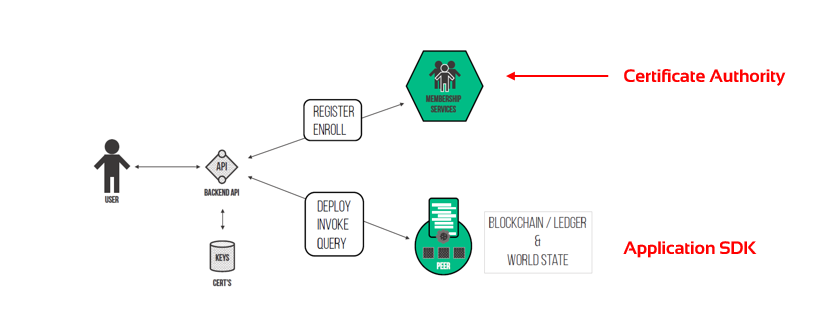
\includegraphics[scale=0.90]{figures/06.png}
	\caption{Whistle Blower Sign up }
	\label{fig:istl}
\end{figure}  
The Hyperledger Fabric CA is a Certificate Authority (CA) for Hyperledger Fabric.\\
It provides features such as:
\begin{itemize}
	\item	registration of identities, or connects to LDAP as the user registry 
	\item 		issuance of Enrollment Certificates (ECerts)
	\item 		certificate renewal and revocation
\end{itemize}
The figure below (see \figref{istb}) shows Certificate Authority Architecture.\\ 
\begin{figure}[h]
	\centering
	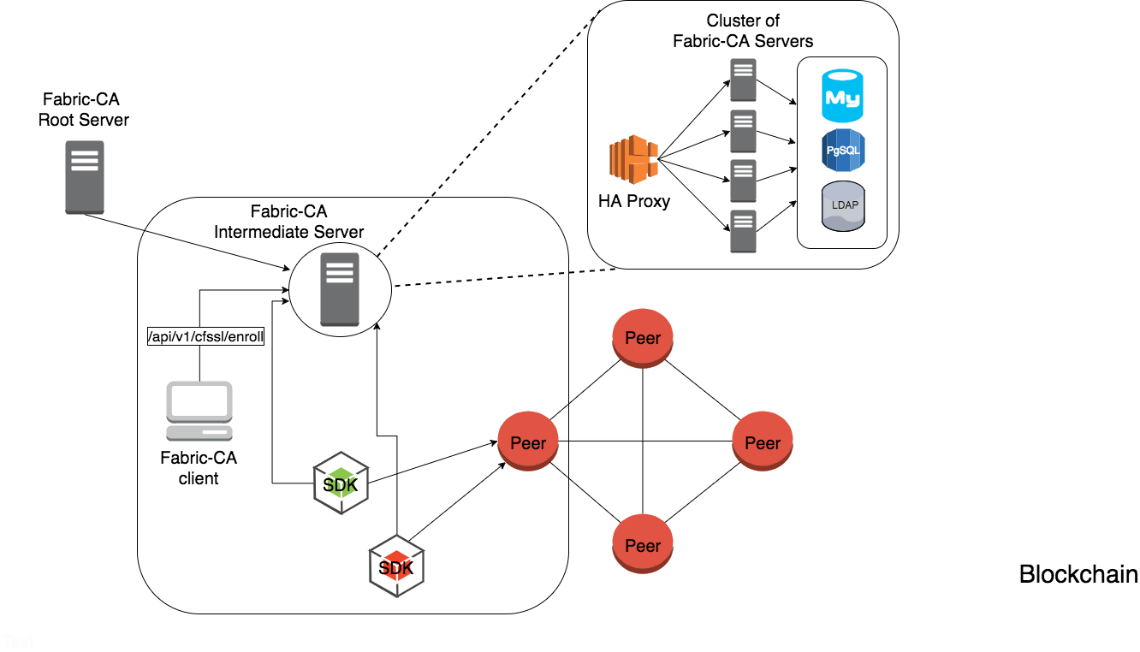
\includegraphics[scale=0.90]{figures/07.png}
	\caption{Certificate Authority Architecture }
	\label{fig:istb}
\end{figure}  
\begin{itemize}
	\item	Interact with application
	\item 	Invoke the smart contract (Any request you put through)\\
	\textbf{      Updating Status }-Suppose you visited the after few days and a new evidence is found. If the case is solved, The Judge will change the status to solve. 
	\item 		Updating the distributed ledger 
		after the action will happen the distributed ledger will get updated. The consensus mechanism whether approve or disapprove your request a new block is added into the system.\\ 
		If the block is approved the world state of ledger will change else the world state will remain the same. 
	
\end{itemize}
The figure below (see \figref{istz}) shows Whole Whistle-blower Architecture.\\ 
\begin{figure}[h]
	\centering
	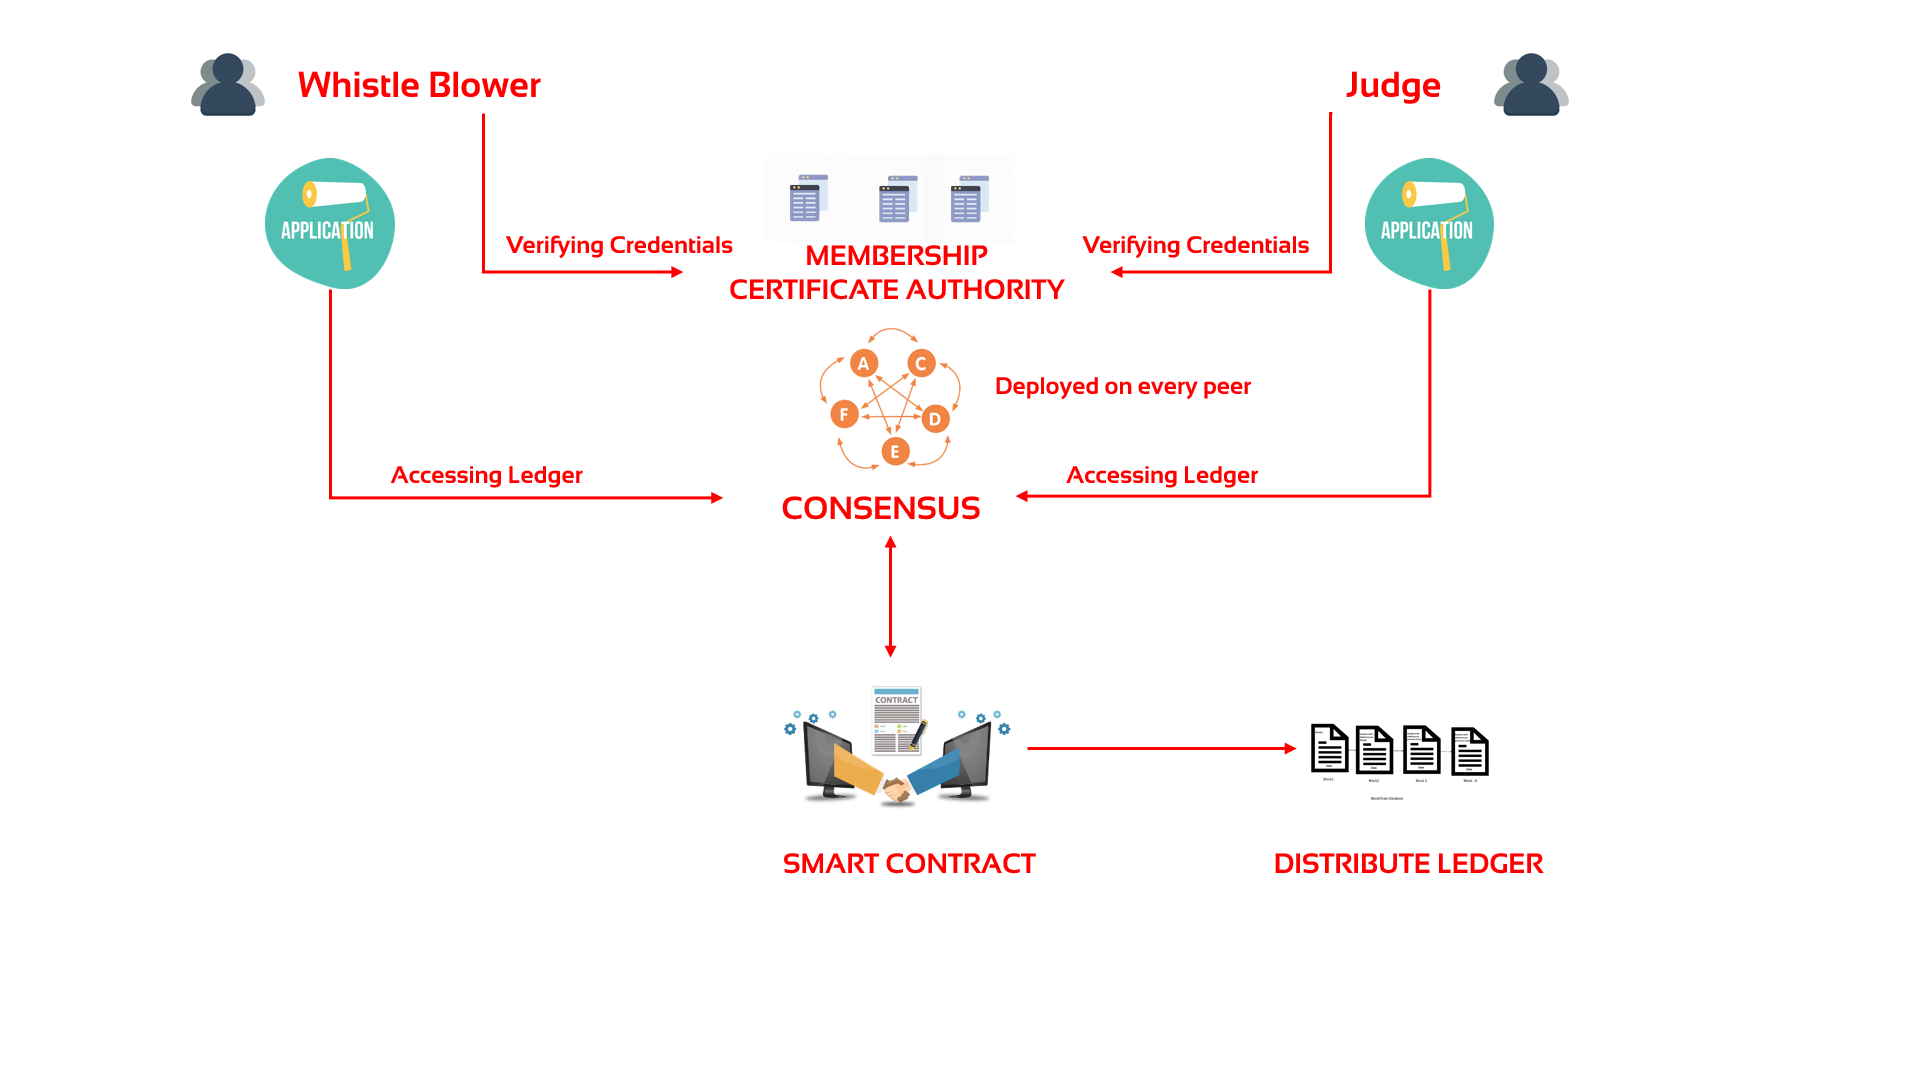
\includegraphics[scale=0.40]{figures/08.png}
	\caption{Whistle-blower Architecture }
	\label{fig:istz}
\end{figure}  
\section{Workflow of few Use Cases Together }
\subsection{Use Cases}
\subsubsection{Web Interface}
First you have to open the Front End of the application (Website) and see cases. Different cases will be uploaded there.
If you have any information regarding that you have to go and register on a whistle blower page
\subsubsection{Register a Whistle Blower}
It will not ask for your NIC or anything. You can register using a fake name and wallet. But in case you need reward wallet number can be put correctly and will not get trace back to you. One registration means one block is added into the system. Then you can submit an evidence to a case or report any illegal activity happening in the country.
\subsubsection{Discuss with Police}
The police can view all the cases and evidence and can submit their own. You can also discuss cases with the police and let’s see what their opinion about that case is. 
\subsubsection{Agency/Judge}
They are like few people 10-30 handling the system selected randomly to avoid them being get corrupted. The will also monitor police activities and their decisions over all the cases.  
\subsubsection{Blockchain Backend Working}
When a transaction is done all the peers node will see it and the consensus algorithm will take place. If it gets validated means the transaction is added in the ledger and it will change the world state of the blockchain.\\ 
If it’s not get validated it will still record that action that some subscriber tried this. It will be stored in the ledger but world state of blockchain is not updated.
The figure below (see \figref{istf}) shows the Work-flow diagram.\\ 
\begin{figure}[h]
	\centering
	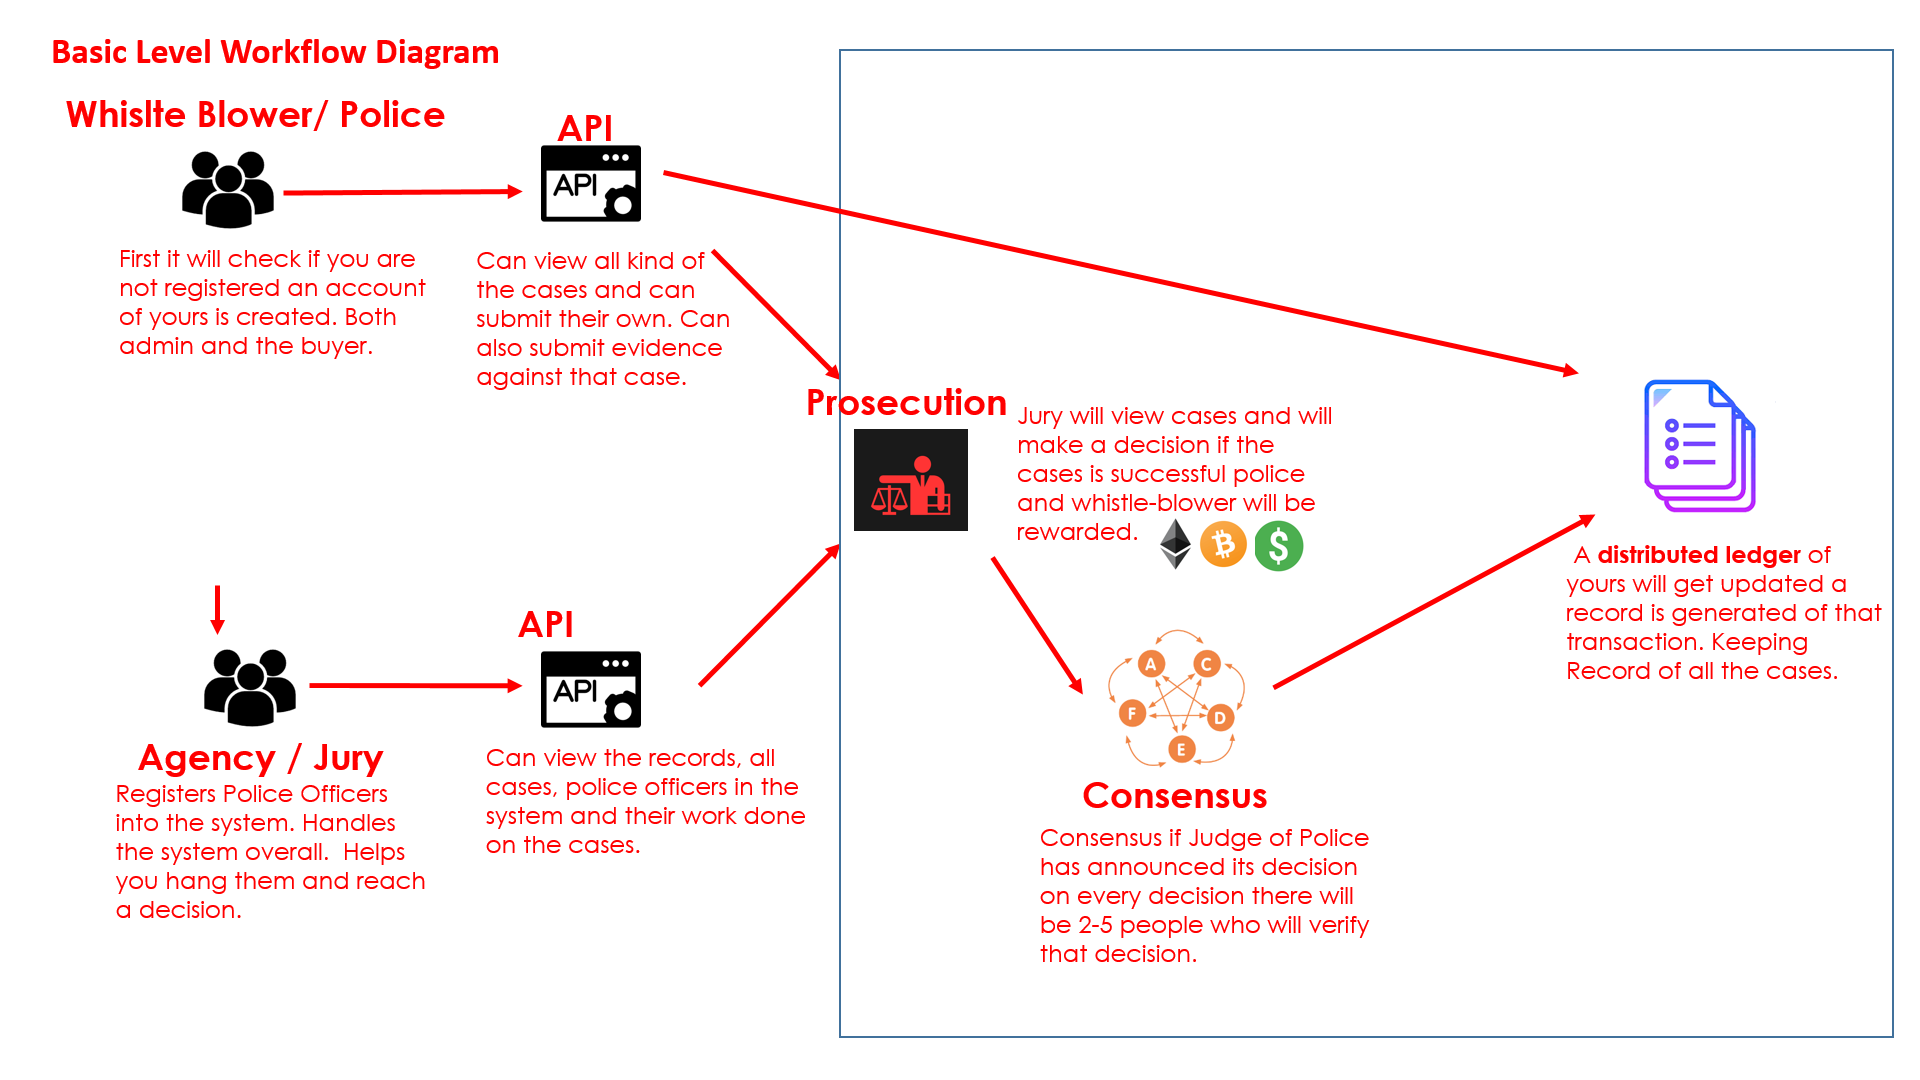
\includegraphics[scale=0.40]{figures/09.png}
	\caption{Work-flow diagram }
	\label{fig:istf}
\end{figure} 